\subsection{The \mkpimm invariant mass distribution}
\label{sec:kpimm:massfit}

The $m(\Kp\pim\mumu)$ invariant mass is used to discriminate between signal and background. The signal distribution is modelled using the sum of two Gaussian functions with a common mean, each with a power-law tail on the low-mass side.  The combinatorial background is modelled using an exponential function.  The parameters describing the shape of the mass distribution of the signal are determined from a fit to the \BdToJPsiKstP decay in data, as shown in Fig.~\ref{fig:massfit:jpsi}, and are subsequently fixed when fitting the \BdToKpimm candidates. An additional component is included to model the contribution from \BsToJPsiKst in the fit to the control mode. 

\begin{figure}[!tb]
\centering
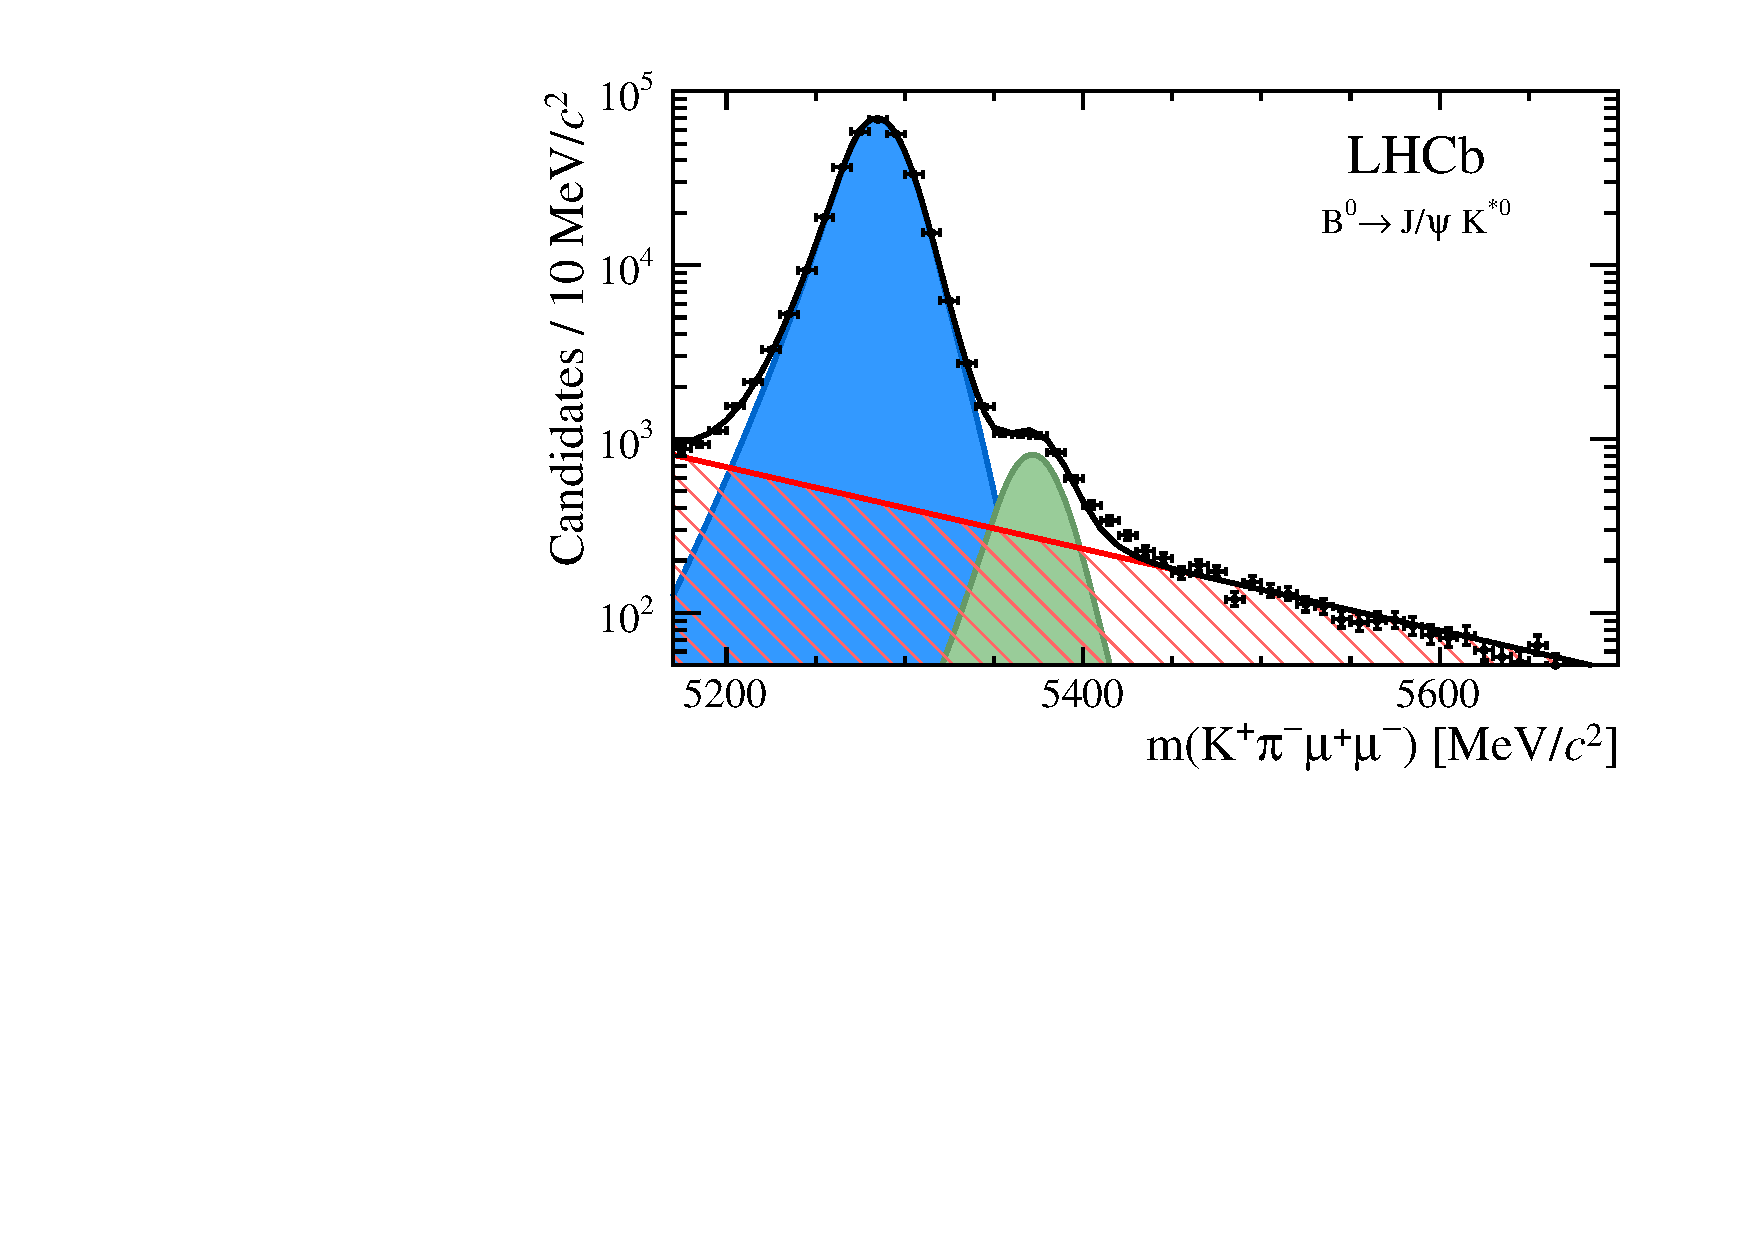
\includegraphics[width=0.7\linewidth]{figs/kpimm/massfit/fit_jpsi_log.pdf}
\caption{Invariant mass \mkpimm for the control decay \BdToJPsiKst. The solid black line represents the total fitted function.  The individual components of the \BdToJPsiKst (blue shaded area), \BsToJPsiKst (green shaded area) and combinatorial background (red hatched area) are also shown.}
\label{fig:massfit:jpsi}
\end{figure}

A single scaling factor is used to correct the width of the Gaussian functions to account for variations in the shape of the mass distribution of the signal observed in simulation, due to the different regions of \mkpi and \qsq between the control mode and signal mode. This factor is determined by first fitting the \mkpimm distribution for simulated four-body \BdToKpimm decays in the \BdToJPsiKstP region.  All the fit parameters are then fixed, except for $s_{\sigma}$ which is allowed to float in the subsequent fits to the \mkpimm distribution in each of the \qsq bins in the \BdToKpimm signal region. The distribution of $s_{\sigma}$ as a function of \qsq in the $1330<\mkpi<1530$\mevcc region is shown in Fig.~\ref{fig:massfit:scale}.  %The numerical values are given in Tab.~\ref{tab:massfit:scale}. 

In order to cross-check the method, the scaling factor is determined both for simulated four-body \BdToKpimm decays and for data in the region $9.22<\qsq<9.96\gevgevcccc$ and $1330<\mkpi<1530\mevcc$.  The value of $s_{\sigma}$ determined from simulation is in good agreement with that determined from data.

\begin{figure}[!tb]
 \centering
 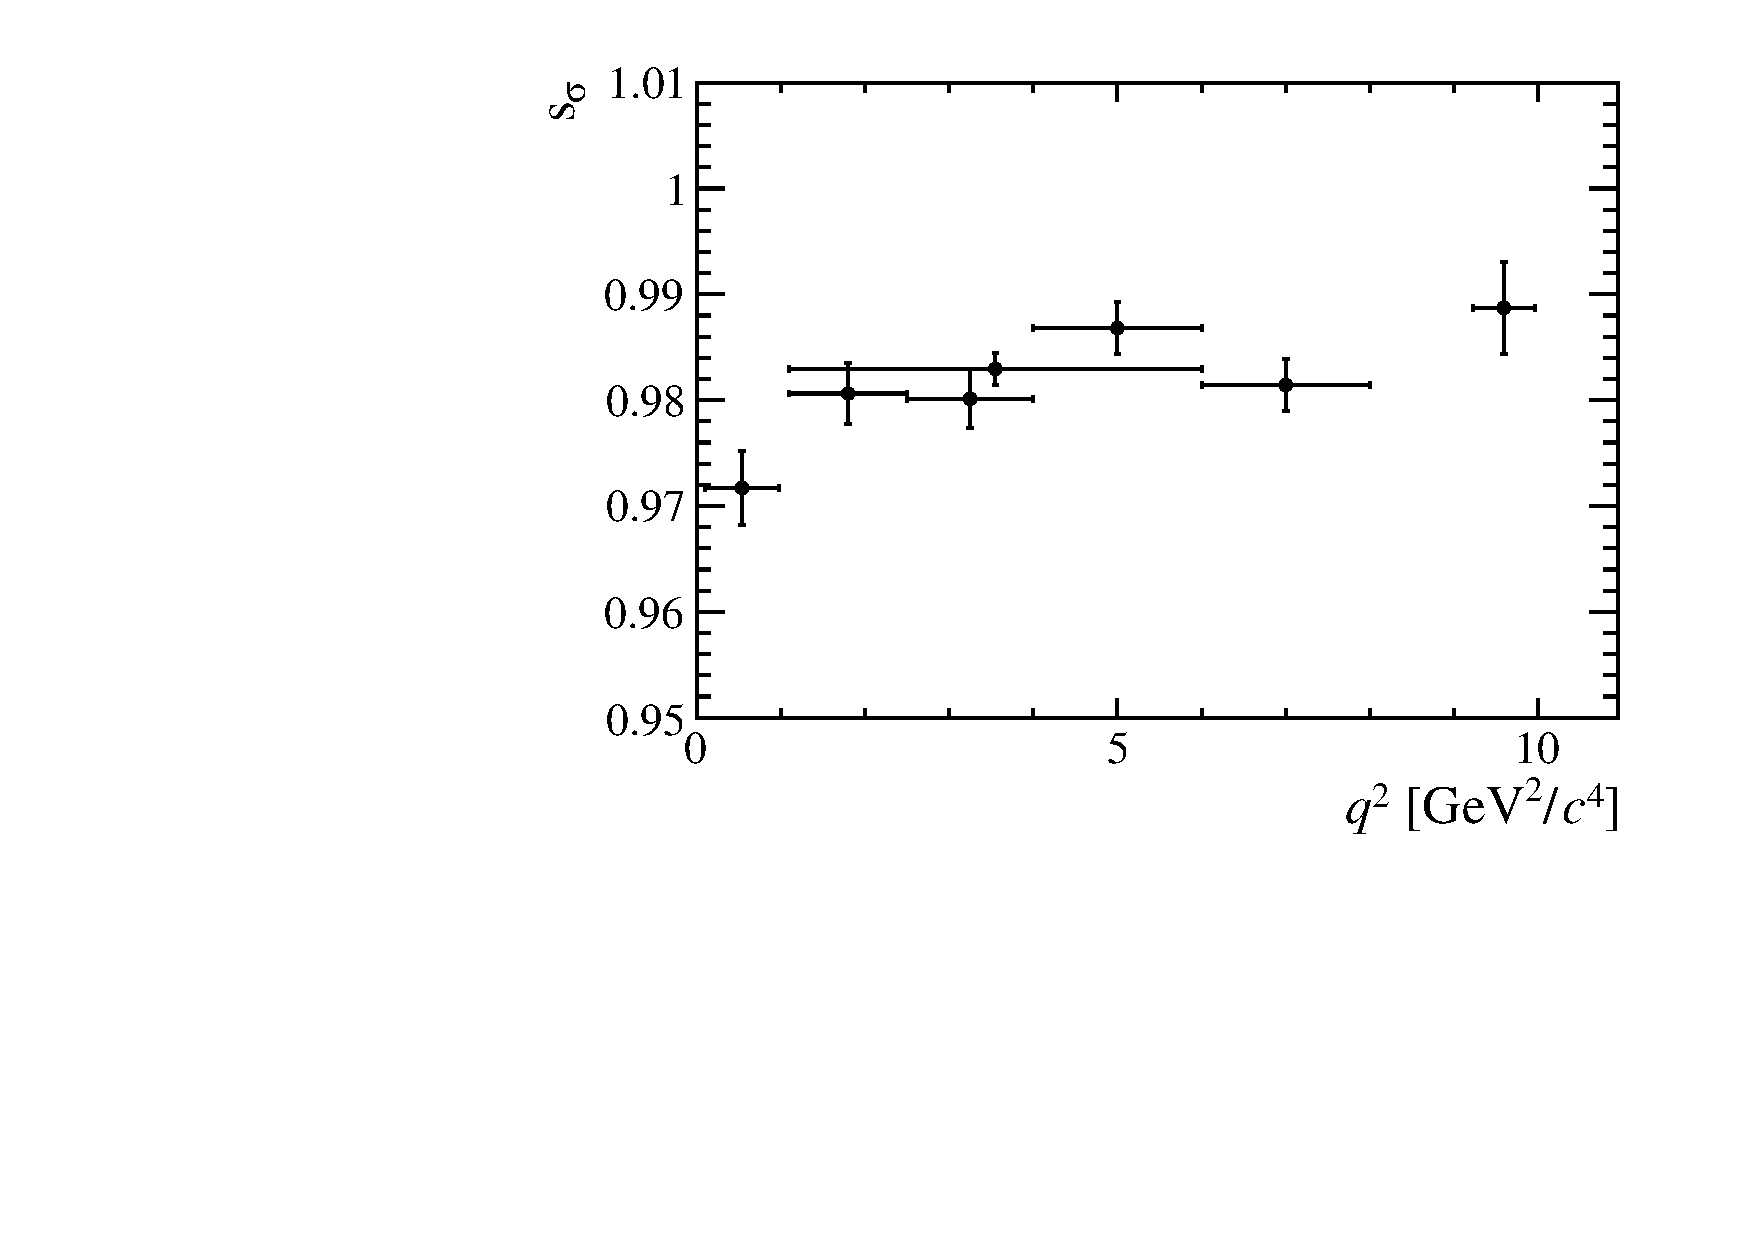
\includegraphics[width=0.7\textwidth]{figs/kpimm/massfit/s_sigma.pdf}
 \caption{Scaling factor $s_{\sigma}$ in bins of \qsq for candidates in the $1330<\mkpi<1530$~\mevcc region.
 \label{fig:massfit:scale}}
\end{figure}

% \begin{table}[!tb]
% \begin{center}
% \begin{tabular}{lc}
% \qsq [\gevgevcccc] & Scaling factor \\
% \hline
% $[0.10,0.98]$ & 0.972 $\pm$ 0.004 \\
% $[1.10,2.50]$ & 0.981 $\pm$ 0.003 \\
% $[2.50,4.00]$ & 0.980 $\pm$ 0.003 \\
% $[4.00,6.00]$ & 0.987 $\pm$ 0.002 \\
% $[6.00,8.00]$ & 0.981 $\pm$ 0.002 \\
% \hline
% $[1.10,6.00]$ & 0.983 $\pm$ 0.002 \\
% \hline
% $[9.22,9.96]$ & 0.989 $\pm$ 0.004 \\
% \end{tabular}
% \caption{Scaling factor $s_{\sigma}$ in bins of \qsq for candidates in the $1330<\mkpi<1530$~\mevcc region.
% \label{tab:massfit:scale}}
% \end{center}
% \end{table}

 The fit to \BdToKpimm candidates in the range $1.1 < \qsq < 6.0\gevgevcccc$ is shown in Fig.~\ref{fig:massfit:kpimm}.  The individual fits to the \BdToKpimm candidates in each of the \qsq bins used for the differential branching fraction measurement are shown in Appendix~\ref{sec:appendix:massfit}. The signal and background yields in each of the \qsq bins in the range $5170<\mkpimm<5700$~\mevcc are given in Table~\ref{tab:massfit:yields}.

\begin{figure}[!tb]
\centering
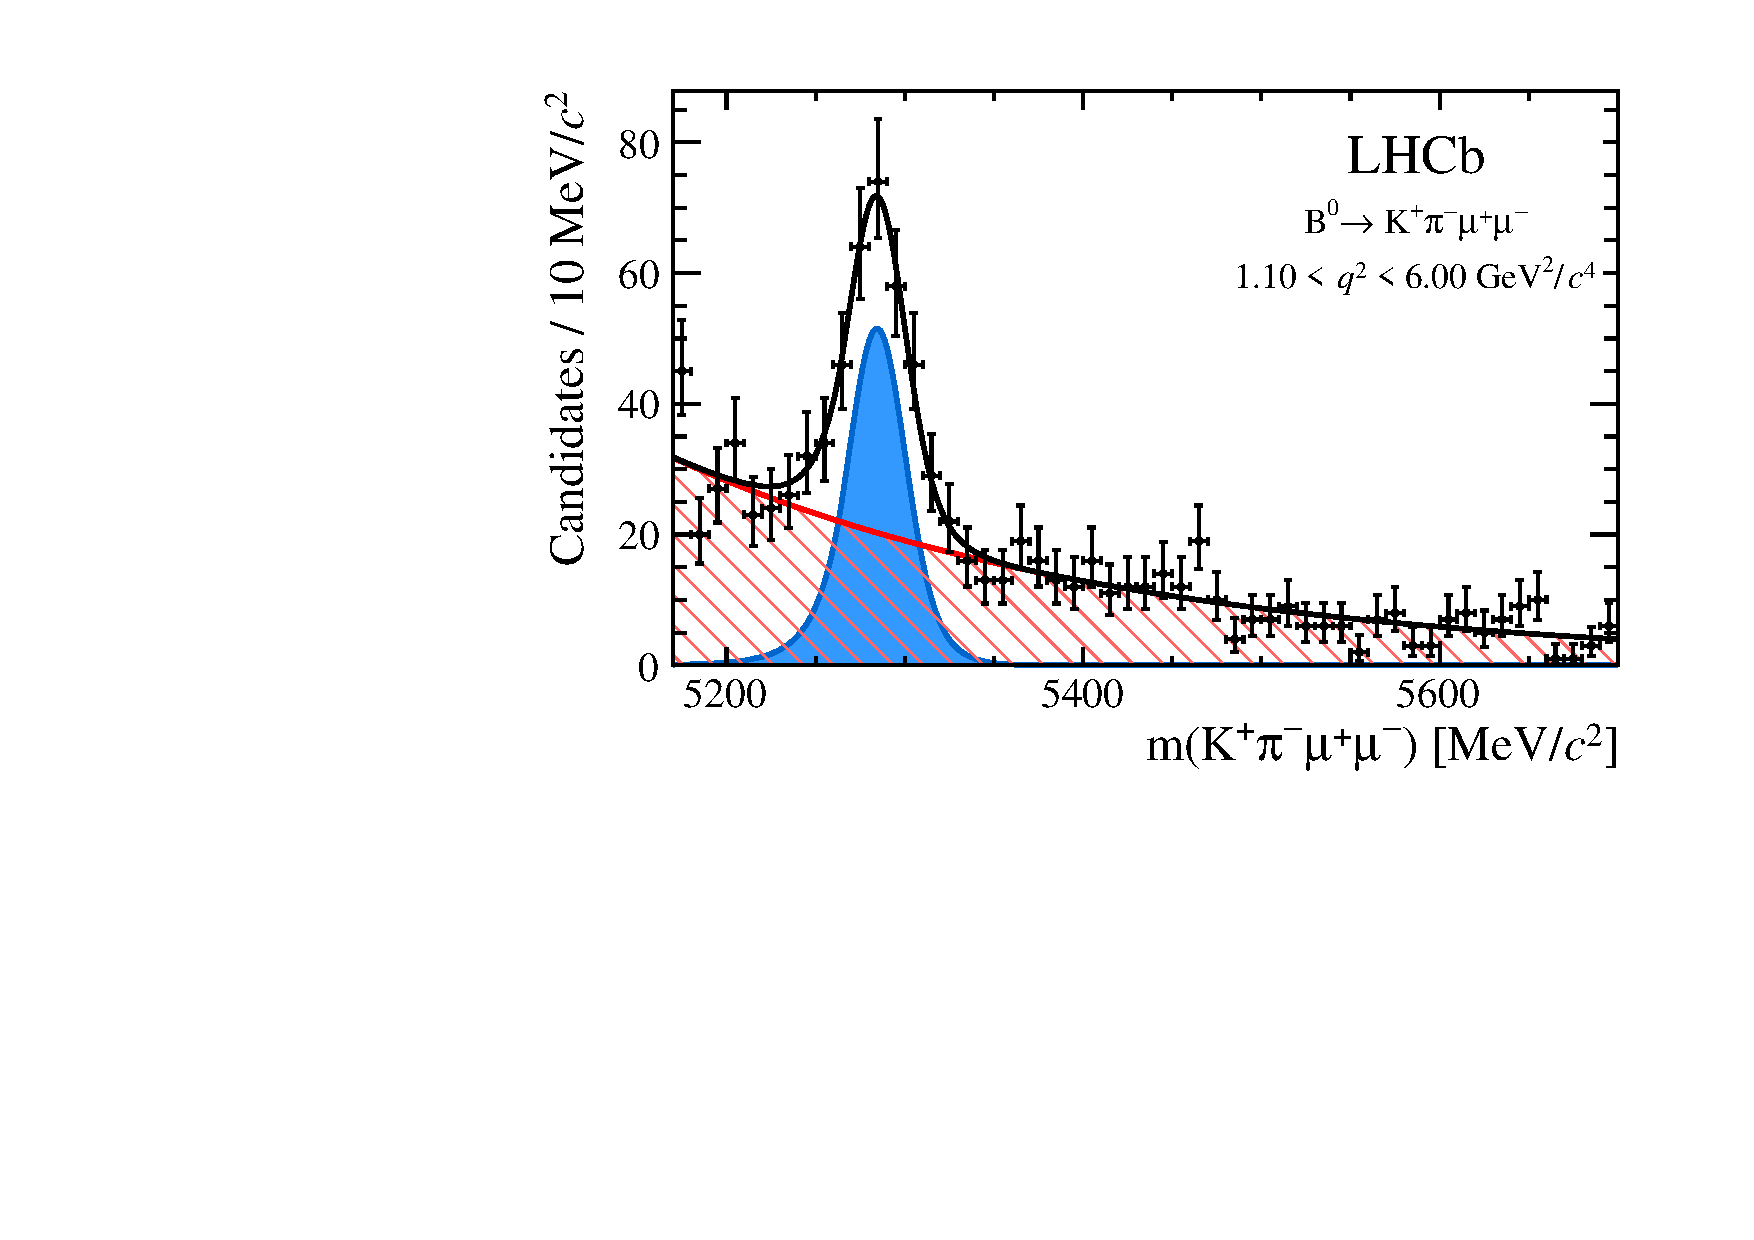
\includegraphics[width=0.7\linewidth]{figs/kpimm/massfit/fitKpimumu_q2_1p1_6p0.pdf}
\caption{Invariant mass \mkpimm for the signal decay \BdToKpimm in the range $1.1 < \qsq < 6.0\gevgevcccc$. The solid black line represents the total fitted function.  The individual components of the signal (blue shaded area) and combinatorial background (red hatched area) are also shown.}
\label{fig:massfit:kpimm}
\end{figure}

\begin{table}[!htb]
\begin{center}
\begin{tabular}{lcc}
\qsq [\gevgevcccc] & Signal yield & Background yield \\
\hline
$[0.10,0.98]$ & 67 $\pm$ 10 & 93 $\pm$ 11 \\
$[1.10,2.50]$ & 80 $\pm$ 12 & 160 $\pm$ 15 \\
$[2.50,4.00]$ & 75 $\pm$ 12 & 213 $\pm$ 17 \\
$[4.00,6.00]$ & 75 $\pm$ 13 & 334 $\pm$ 21 \\
$[6.00,8.00]$ & 60 $\pm$ 14 & 476 $\pm$ 25 \\
\hline
$[1.10,6.00]$ & 229 $\pm$ 21 & 708 $\pm$ 31 \\
\end{tabular}
\caption{Signal and background yields of the \BdToKpimm candidates in each of the \qsq bins.
\label{tab:massfit:yields}}
\end{center}
\end{table}